\chapter{Ergebnisse}\label{ergebnisse}

\section{Nutzbarkeit der SYCL-Implementierungen}
\label{ergebnisse:nutzbarkeit}

Im Folgenden wird die Nutzbarkeit von drei öffentlich verfügbaren
SYCL"=Implementierungen dargelegt. Dabei handelt es sich um ComputeCpp sowie
die Implementierungen der Firmen Intel und Xilinx. Die im Kapitel~\ref{sycl}
erwähnten Implementierungen hipSYCL und sycl-gtx wurden während dieser Arbeit
nicht in Betracht gezogen, da ihnen zu viele kritische Features fehlen und sie
daher nicht für eine Nutzung mit Alpaka geeignet sind.

\subsection{ComputeCpp}

Die folgenden Ausführungen zu ComputeCpp beziehen sich auf die frei verfügbare
\textit{Community Edition} und alle Versionen bis einschließlich Version 1.1.5.

Von den derzeit der Öffentlichkeit zugänglichen SYCL"=Implementierungen ist
ComputeCpp die einzige, die nicht quelloffen ist. Sie wird vom schottischen
Unternehmen Codeplay entwickelt, welches ebenfalls federführend an der
Entwicklung des SYCL"=Standards beteiligt ist. ComputeCpp unterstützt mehr
Hardware"=Plattformen als die anderen SYCL"=Implementierungen.

Im Laufe der Implementierung des SYCL"=Backends stellte sich schnell heraus,
dass ComputeCpp nicht in der Lage sein würde, das SYCL"=Alpaka"=Backend zu
verwenden. Dafür gibt es zwei Gründe, die nachstehend weiter ausgeführt werden.

\subsubsection{Zeiger}

Zusätzlich zu der in Kapitel~\ref{implementierung} beschriebenen Problematik
mit Zeigern kommt es zu weiteren Schwierigkeiten, wenn Zeiger in Verbindung mit
ComputeCpp genutzt werden sollen.

ComputeCpp versucht die Information, zu welchem Adressraum ein Zeiger gehört,
durch spezielle Zeiger"=Attribute nachzuliefern. Ein Zeiger des Typs
\texttt{int*}, der auf den globalen Adressraum zeigt, wird vom
ComputeCpp"=Compiler zu \texttt{\_\_global int*} transformiert. Das Ergebnis der
Transformation wird vom selben Compiler jedoch als ein eigener Typ betrachtet,
der nichts mehr mit \texttt{int*} zu tun hat. Dadurch kommt es zu Problemen mit
den \textit{type traits} der C++"=Standardbibliothek, die einen Zeiger vom Typ
\texttt{\_\_global int*} nicht mehr als \texttt{int}"=Zeiger erkennen.

Da es dem Programmierer ebenfalls verboten ist, diese Attribute selbst zu
verwenden (ComputeCpp generiert einen Syntax"=Fehler), kann eine manuelle
Auswahl entsprechender Code"=Pfade nicht vorgenommen werden.

Darüber hinaus sind diese Zeigertypen nicht mit den SYCL"=Klassen kompatibel.
So führt die Umwandlung eines entsprechenden Zeigers in einen
SYCL"=\texttt{multi\_ptr} dazu, dass letzterer nicht mehr mit den atomaren
Funktionen des SYCL"=Standards verwendet werden kann. In diesem Fall meldet
ComputeCpp den Fehler, dass die Verwendung von Adressraum"=Attributen in
Verbindung mit atomaren Funktionen verboten ist.

\subsubsection{Fehlerhafte Instruktionen}

Auf NVIDIA"=GPUs generiert ComputeCpp mitunter Instruktionen, die von NVIDIAs
OpenCL"= oder CUDA"=Umgebung nicht verstanden werden. Dies fällt erst bei der
Ausführung des Kompilats auf, das entsprechende Fehlermeldungen der
NVIDIA"=Laufzeitumgebung meldet. Darüber hinaus fehlen ComputeCpp noch einige
wichtige Instruktionen, die für ein Funktionieren mit Alpaka nötig sind,
darunter viele mathematische Funktionen.

\subsection{Intel}

Eine weitere wichtige Implementierung des SYCL"=Standards wird seit Anfang des
Jahres 2019 von der Firma Intel herausgegeben. Diese quelloffene Variante ist
auf die Nutzung der Intel"=OpenCL"=Umgebungen für CPUs und GPUs ausgelegt. Es
ist aufgrund der parallel zu dieser Arbeit verlaufenen Weiterentwicklung
absehbar, dass kurz"= bis mittelfristig auch die FPGAs dieses Herstellers
unterstützt werden sollen.

Intels Compiler ist die einzige SYCL"=Implementierung, die Alpaka"=Quelltexte
mit aktiviertem SYCL"=Backend kompilieren konnte und kam deshalb zur
Verfizierung zum Einsatz.

\subsection{Xilinx}
\label{ergebnisse:nutzbarkeit:xilinx}

In dieser Arbeit wurde der Entwicklungszweig der Xilinx"=SYCL"=Implementierung
verwendet, der dem Hauptzweig einige Wochen voraus und näher an der zugrunde
liegenden Intel"=Implementierung ist. Die folgenden Ausführungen beziehen sich
auf:

\begin{itemize}
    \item den Commit \#\texttt{dfb95af} des Zweiges \texttt{sycl/unified/next}
          der Xilinx"=Implementierung,
    \item die Entwicklungsumgebung SDAccel 2019.1,
    \item die OpenCL"=Umgebung XRT 2.2 und
    \item die Deployment"=Plattform \texttt{xilinx-u200-xdma} für Ubuntu 18.04
          samt der zugehörigen Entwicklungs"=Plattform
          \texttt{xilinx-u200-xdma-dev} (beide in Version
          \texttt{201830.2-2580015}) für den Beschleuniger Alveo U200.
\end{itemize}

Die SYCL"=Implementierung der Firma Xilinx hängt eng mit der Entwicklung des
Intel"=SYCL"=Compilers zusammen. Dabei wird in unregelmäßigen Abständen die
Code"=Basis des Intel"=Compilers übernommen und die Xilinx"=eigenen Codepfade
darin integriert. Das hat zur Folge, dass Fehlerkorrekturen des Intel"=Compilers
erst mit einiger Verzögerung in die Xilinx"=Implementierung Eingang finden.

Darüber hinaus erwies sich die Schnittstelle des SYCL"=Compilers zu Xilinx'
SDAccel"=Plattform, welche die eigentliche Synthese durchführt, sowie zu Xilinx'
OpenCL"=Treibern im Laufe dieser Arbeit als fehleranfällig und unvollständig.
Aufgrund dieser Probleme war eine Nutzung des Alpaka"=SYCL"=Backends für
Xilinx"=FPGAs nicht möglich.

\subsubsection{Mathematische Funktionen}

Der Compiler generiert aus einigen mathematischen SYCL"=Funktionen
Instruktionen, die in Xilinx' OpenCL"=Treiber nicht vorhanden sind. Dies ist
zwar auf ein falsches Benennungsschema innerhalb der OpenCL"=Implementierung
zurückzuführen, steht einer Nutzbarkeit im Zusammenhang mit Alpaka aber trotzdem
im Wege. Andere mathematische Funktionen (z.B. \texttt{rsqrt(double)}) führen
unter ungünstigen Umständen durch ihre Nutzung dazu, dass der Compiler selbst
abstürzt.  

\subsubsection{Strukturen}

Zu einem gravierenden Problem kommt es bei der Nutzung von benutzerdefinierten
Strukturen. Werden diese außerhalb eines Kernels definiert und dann innerhalb
eines Kernels verwendet, kommt es zu einem Absturz des Compilers. Der Grund
dafür liegt in einem Fehler des im Hintergrund verwendeten
Xilinx"=OpenCL"=Compilers \texttt{xocc}, welcher die Synthese steuert. Nach
Aussage der an der SYCL"=Implementierung beteiligten Xilinx"=Mitarbeiter genießt
die Behebung dieses Fehlers niedrige Priorität, weshalb in nächster Zeit nicht
mit Besserung zu rechnen ist (siehe
Anhang~\ref{anhang:diskussionen:xilinx:knownissues}). Dieser Fehler ist der
hauptsächliche Grund, warum das aus vielen Strukturen bestehende Alpaka nicht
mit Xilinx' SYCL"=Implementierung verwendet werden kann.

\subsection{Block RAM und Pipelining}

In Xilinx' OpenCL"=Implementierung wird \textit{local memory} in Block RAM
synthetisiert, um den Logikblöcken möglichst schnelle Speicherzugriffe bieten zu
können. Xilinx' SYCL"=Implementierung verfügt ebenfalls über die notwendigen
Klassen und Strukturen, um \textit{local memory} innerhalb eines
\textit{Kernels} verwenden zu können. Aufgrund eines Compiler"=Fehlers werden
diese jedoch nicht als solche erkannt, wodurch Felder im \textit{local memory}
tatsächlich im \textit{global memory} angelegt werden.

Alternativ ließe sich Block RAM über die in
Abschnitt~\ref{sycl:erweiterungen:xilinx:partitioning} erwähnten
SYCL"=Erweiterungen für die Feldpartitionierung verwenden. Diese sind jedoch
ebenfalls vom oben genannten Problem mit \textit{kernel}"=fremden Strukturen
betroffen und führen zu einem Compiler"=Absturz.

Zusammengefasst lässt sich Block RAM mit keiner der in SYCL dafür vorgesehenen
Funktionalität nutzen. Dies wirkt sich auch auf die Nutzung der Erweiterung
für Pipelining aus. Ein häufiges Speicherzugriffsmuster bei FPGAs sind die
\textit{burst reads} genannten Speicherzugriffe. In einer Schleife werden
aufeinander folgende Daten -- z.B. eine Pixelzeile eines Bildes -- vom
\textit{global memory} in den \textit{local memory} kopiert. Durch die Anwendung
des Pipelining"=Prinzips auf diese Schleife lässt sich die zur Verfügung
stehende Bandbreite besser ausnutzen, als wenn erst im eigentlichen Algorithmus
auf die Daten des \textit{global memory} zugegriffen würde.

Da der \textit{local memory} nicht zur Verfügung steht, erfolgen Lese"= und
Schreibzugriffe ausschließlich auf den \textit{global memory}. Die Zahl der
zugehörigen Lese"= und Schreib"=Ports ist jedoch begrenzt, wodurch die Schleife
nicht dem Pipelining"=Prinzip unterworfen werden kann.

\subsubsection{Kompatibilität mit der SDAccel"=Umgebung}

Zur Generierung von Profiling"=Informationen während der Hardware"=Emulation ist
es notwendig, die ausführbare Datei mit Debug"=Symbolen zu generieren
(Compiler"=Flag \texttt{-g}). Durch einen Compiler"=Fehler werden allerdings im
\textit{Kernel}"=Kompilat inkompatible Debug"=Symbole generiert, die von Xilinx'
OpenCL"=Umgebung nicht verarbeitet werden können. Das macht die Nutzung des
mitgelieferten visuellen Profilers \texttt{sdx} bzw. die Visualisierung der
Profiling"=Ergebnisse in Form von Timelines unmöglich.

\subsubsection{OpenCL-Treiber}

Xilinx' OpenCL"=Treiber, auf dem die SYCL"=Implementierung aufsetzt, erwies sich
im Zusammenspiel mit SYCL als äußerst instabil. Aufgrund seiner internen
Struktur ist er nicht in der Lage, einmal reservierten Speicher wieder
freizugeben, wenn das reservierende Programm abstürzt. Der Speicher bleibt so
lange unzugänglich, bis der Treiber neu gestartet wird. Da dies nur mit
Administrationsrechten funktioniert, ist dies de facto ein Ausschlusskriterium
für den Einsatz in Rechenzentren oder Hochleistungs"=Clustern.

Sofern der Treiber nicht das oben beschriebene Verhalten zeigt, kann ein
fehlerhaftes Programm auch zum Komplettabsturz des Gesamtsystems führen. In
diesem Fall ist das System per Fernzugriff nicht mehr erreichbar und muss
vom Administrator (oder physisch per Reset"=Taste) neu gestartet werden. Für den
Einsatz in Rechenzentren und vergleichbaren Einrichtungen ist dieses
Fehlerverhalten denkbar ungeeignet.

\subsection{Zusammenfassung}
 
Von den beschriebenen SYCL"=Implementierungen konnte nur der Intel"=Compiler im
Zusammenhang mit Alpaka genutzt werden, was als Ziel"=Hardware für das
SYCL"=Backend nur Intel"=CPUs und -GPUs zulässt. Insbesondere Xilinx"=FPGAs
können zum aktuellen Zeitpunkt aufgrund zahlreicher Probleme der
SYCL"=Implementierung nicht vom Alpaka"=SYCL"=Backend verwendet werden.

\section{Vergleich zwischen Alpaka und SYCL}

Im direkten Vergleich erwies sich SYCL gegenüber Alpaka als die modernere,
intuitivere und angenehmer zu benutzende Schnittstelle.

Dazu tragen SYCLs Orientierung an modernen C++"=Standards (alle untersuchten
Implementierungen unterstützen den C++17"=Standard, Intel und Xilinx darüber
hinaus den in Entwicklung befindlichen C++20"=Standard) sowie die stilistische
Nähe zur C++"=Standardbibliothek bei. Dem gegenüber stehen Alpakas
Stil"=Konventionen, die vom in der C++"=Standardbibliothek verwendeten
\textit{snake case} (\texttt{eine\_kleine\_funktion()}) zugunsten des
\textit{lower camel case} (\texttt{eineKleineFunktion()}) abweichen. Darüber
hinaus finden sich in Alpaka stilistische Eigentümlichkeiten, die in den meisten
C++"=Projekten unüblich sind, z.B. die Schreibweise als \texttt{char const *}
anstelle des weiter verbreiteten \texttt{const char *}. Damit weicht das
C++"=Projekt Alpaka auch von den vom C++"=Standardisierungskomitee
veröffentlichen Stilrichtlinien ab, den \textit{C++ Core Guidelines}.

Die Modellierung von Aufgabengraphen bzw.\ der Abhängigkeiten zwischen Kerneln
ist in SYCL deutlich einfacher als in Alpaka. Während dies in SYCL automatisch
von der Laufzeitumgebung übernommen wird, muss der Programmierer in Alpaka
selbst tätig werden -- der Aufwand ist in Alpaka also höher.

Die meisten Konzepte sind in SYCL und Alpaka jedoch recht ähnlich, sodass
hinsichtlich der Mächtigkeit keine großen Unterschiede bestehen. Darüber hinaus
hat Alpaka gegenüber SYCL den faktischen Vorteil der Hardware"=Unterstützung.
Während SYCL zur Zeit nur mit Intel"=CPUs und -GPUs zufriedenstellend
funktioniert (und möglicherweise nicht getesteter Automotive"= und
Embedded"=Hardware), ist Alpaka auf NVIDIA"= und AMD"=GPUs sowie über OpenMP auf
allen CPUs lauffähig. Daher ist Alpaka bereits in einigen produktiven
Anwendungen im Einsatz, während sich SYCLs Ökosystem bislang auf diverse
Implementierungen sowie einige von der Firma Codeplay entwickelte Bibliotheken
für Mathematik und neuronale Netzwerke beschränkt. 

\section{Verifizierung des SYCL-Alpaka-Backends}
\label{ergebnisse:verifizierung}

Als Integrationstest für das SYCL"=Backend diente das in Alpaka geschriebene
Programm \textit{jungfrau"=photoncounter}, das von der Gruppe
\textit{Computergestützte Strahlenphysik} des \textit{Instituts für
Strahlenphysik} am \textit{Helmholtz"=Zentrum Dresden"=Rossendorf} in
Zusammenarbeit mit dem schweizerischen
\textit{Paul Scherrer Institut}\footnote{Sic! Das PSI schreibt sich ohne
Bindestriche.} (PSI) entwickelt wird und 2018 in Sebastian Benners
Bachelorarbeit beschrieben wurde \cite[vgl.][]{benner2018}.

\subsection{Der \textit{jungfrau-photoncounter}}
\label{ergebnisse:verifizierung:jungfrau}

Der \textit{jungfrau"=photoncounter} wertet Daten des Photonendetektor"=Typs
JUNGFRAU (\textit{ad\textbf{ju}sti\textbf{n}g \textbf{g}ain detector
\textbf{f}o\textbf{r} the \textbf{A}ramis \textbf{u}ser station}) aus und zählt
die von diesem registrierten Photonen. Der JUNGFRAU"=Detektortyp wird für den am
PSI befindlichen Freie"=Elektronen"=Laser \textit{SwissFEL} entwickelt. Ein
JUNGFRAU"=Detektor verfügt über eine Auflösung von 16 Megapixeln mit 2 Byte pro
Pixel und produziert Messergebnisse mit einer Frequenz von derzeit
\SI{100}{\hertz} (umgerechnet \SI{3.2}{\giga\byte\per\second}). Der Detektortyp
befindet sich nach wie vor in Entwicklung und soll langfristig Daten mit einer
Frequenz von \SI{2.2}{\kilo\hertz} (umgerechnet \SI{74}{\giga\byte\per\second})
generieren. Das macht eine dementsprechend schnelle Weiterverarbeitung der Daten
durch den \textit{jungfrau"=photoncounter} notwendig.

In Rahmen dieser Arbeit wurde nur der Teil des gesamten Funktionsumfangs des
\textit{jungfrau"=photoncounters} betrachtet, der sich mit dem Zählen der
Photonen pro Detektor"=Pixel befasst. Der Algorithmus berechnet für jedes
Detektorpixel die Formel

\begin{equation}\label{ergebnisse:verifizierung:jungfrau:formel}
    N_\gamma = \frac{\text{ADC} - \text{Sockel}}{\text{Verstärkung} \cdot E_\gamma}
\end{equation}
\noindent
Dabei bezeichnet $N_\gamma$ die Zahl der erkannten Photonen, \textit{ADC} das
vom Analogen ins Digitale konvertierte Messergebnis des Pixels, \textit{Sockel}
das von Mess- und Umweltbedingungen abhängige Grundrauschen des jeweiligen
Pixels (engl. \textit{pedestal}), \textit{Verstärkung} die Signalverstärkung
des Pixels (engl. \textit{gain}) und $E_\gamma$ die Photonenenergie.

Um -- im Vergleich zur Multiplikation -- langsame Divisionen bei der Berechnung
zu vermeiden, werden für \textit{Verstärkung} und $E_\gamma$ vor der Ausführung
des Algorithmus die Kehrwerte gebildet. Für $E_\gamma$ kann dies global
erfolgen. Für \textit{Verstärkung} erfolgt die Invertierung mittels eines
eigenen \textit{Kernels} (\texttt{GainmapInversionKernel}), der für jedes Pixel
den Kehrwert bildet.

Der \textit{Sockel}"=Wert wird ebenfalls für jedes Pixel bestimmt. Je nach
Messbedingungen kann er entweder im Abstand einiger Stunden gemessen (z.B. beim
Betrieb des Lasers bei Zimmertemperatur) oder kontinuierlich während der Messung
aktualisiert (z.B. beim Betrieb bei Temperaturen unter dem Gefrierpunkt, da hier
die Pixel empfindlicher sind) werden. Der zweite Fall wird durch einen weiteren
\textit{Kernel} (\texttt{CalibrationKernel}) abgedeckt, der anhand der
Standardabweichung und des Durchschnitts der zuletzt betrachteten Messergebnisse
und \textit{Sockel}"=Werte einen neuen \textit{Sockel}"=Wert berechnet.

Die Formel~\ref{ergebnisse:verifizierung:jungfrau:formel} wird in einem eigenen
\textit{Kernel} umgesetzt (\texttt{PhotonFinderKernel}), der auf jedes vom
Detektor produzierte Messergebniss angewendet wird.

\subsection{Verifizierung und Performanz}
\label{ergebnisse:verifizierung:performanz}

Das SYCL"=Alpaka"=Backend wurde mit dem Commit \#\texttt{78d9957} des
\texttt{sycl}"=Zweigs des Intel"=SYCL"=Compilers in Kombination mit der
\textit{Intel Graphics Compute Runtime for OpenCL} in der Version 19.46.14807
verifiziert. Dabei wurde eine integrierte GPU des Typs \textit{Intel HD Graphics
520} (auch als \textit{Skylake GT2} bezeichnet) als Hardware"=Plattform
verwendet, die über \SI{6}{\gibi\byte} Speicher verfügen kann. Diesen muss sie
jedoch mit dem \textit{Host}"=System teilen. Diese GPU erreicht eine maximale
Performanz von \num{100.8} GFLOPS bei doppelter Präzision\footnote{Die doppelte
Präzision wird innerhalb des Programms benötigt, da einige Zwischenergebnisse in
diesem Format gespeichert werden.}. Das \textit{Host}"=System selbst verfügt
über insgesamt \SI{8}{\gibi\byte} Speicher und ist mit einem Intel"=Prozessor
des Typs i7-6500U ausgestattet, der eine maximale Taktfrequenz von
\SI{3.1}{\giga\hertz} erreichen kann. Als Betriebssystem kam Ubuntu 19.10 zum
Einsatz.

Der Quelltext des \textit{jungfrau"=photoncounters} wurde dem
\texttt{master}"=Zweig des Projekts entnommen (Commit \#\texttt{d94f836}) und
geringfügig an das SYCL"=Backend angepasst. Dabei wurden keine Optimierungen der
\textit{Kernel} für Intel"=Hardware vorgenommen. Von den Entwicklern des
\textit{jungfrau"=photoncounters} wurde für die Messungen der Datensatz mit der
Bezeichung \texttt{px\_101016} zur Verfügung gestellt, der \num{10000}
Messungen mit jeweils $1024 \times 512$ Pixeln umfasst. Aufgrund der
Speicherlimitierung des Gesamtsystems wurde der Datensatz auf \num{1000}
Messergebnisse reduziert.

Die Abbildung~\ref{ergebnisse:verifizierung:performanz:photonen} zeigt das
Ergebnis des oben beschriebenen Algorithmus für den reduzierten Datensatz. Die
weißen Pixel zeigen ungültige Messergebnisse an. Diese werden im
\textit{jungfrau"=photoncounter} durch eine separate Maske eigentlich
abgeschaltet. Durch einen Fehler unbekannter Herkunft funktionierte dieser Teil
des Programms jedoch nicht mit dem Alpaka"=SYCL"=Backend. Der Fehler führt dazu,
dass alle Pixel maskiert werden, was zu einem leeren Ergebnis führt. Aus diesem
Grund wurde auf den Einsatz der Maske verzichtet.

Nach mündlicher Aussage der Entwickler des \textit{jungfrau"=photoncounter} ist
es nicht möglich, die Ergebnisse des im vorigen Abschnitt beschriebenen
Algorithmus anhand synthetischer Daten zu verifizieren. Die Verifizierung realer
Daten erfolgt deswegen durch die Anwender des \textit{Paul Scherrer Instituts},
die die Ergebnisse auf ihre Plausibilität prüfen. Die
Abbildung~\ref{ergebnisse:verifizierung:performanz:photonen} wurde von einem der
Entwickler des \textit{jungfrau"=photoncounter}, Jonas Schenke, für plausibel
befunden.

\begin{figure}
    \centering
    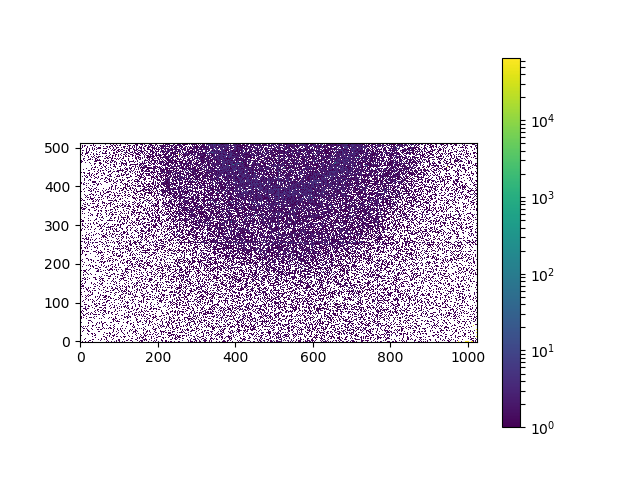
\includegraphics{log/photon.png}
    \caption[Visualisierung eines Ergebnisses des
             \textit{jungfrau-photoncounters}]{Visualisierung eines Ergebnisses
             des \textit{jungfrau-photoncounters}. Weiße Pixel zeigen
             ungültige Ergebnisse an, die nicht maskiert werden konnten.}
    \label{ergebnisse:verifizierung:performanz:photonen}
\end{figure}

Das gezeigte Bild wurde anhand von \num{1000} Messergebnissen berechnet. Die
genannte GPU benötigte für die Verarbeitung der Eingangsdaten (ohne das Laden
der Daten von der Festplatte, Kalibrierung und Invertierung)
\SI{48.372}{\second}. Damit erreicht sie eine Verarbeitungsfrequenz von
\num{20.6731} Messungen pro Sekunde, was unter den derzeitigen \SI{100}{\hertz}
und deutlich unter den avisierten \SI{2.2}{\kilo\hertz} des JUNGFRAU"=Detektors
liegt. Da es sich bei der verwendeten GPU nicht um einen
Hochleistungsbeschleuniger handelt und ihr tatsächlicher Einsatz im Umfeld eines
JUNGFRAU"=Detektors nicht zu erwarten ist, reicht dieses Ergebnis als Beweis
für die grundsätzliche Funktionstüchtigkeit des Alpaka"=SYCL"=Backends aus. In
einem realen Anwendungsszenario wären Beschleuniger mit höherer Leistung
(insbesondere bei doppelter Präzision) zwingend erforderlich, um die angestrebte
Frequenz des JUNGFRAU"=Detektors erreichen zu können.

\subsection{Nutzbarkeit von FPGAs}

Da der Detektor mit fester Frequenz Daten produziert, würde sich ein FPGA für
den beschriebenen Verarbeitungsalgorithmus sehr gut eignen. Durch die in
Abschnitt~\ref{ergebnisse:nutzbarkeit:xilinx} geschilderten Schwierigkeiten
mit der derzeit zur Verfügung stehenden Xilinx"=SYCL"=Implementierung konnte 
das bestehende Alpaka"=Programm jedoch nicht auf Xilinx"=FPGAs zur Ausführung
gebracht werden.

\section{Box-Filter}
\label{ergebnisse:box}

Da sich die ursprünglich für den Einsatz von FPGAs vorgesehene Alpaka"=Anwendung
aufgrund des Entwicklungsstatus der Xilinx"=SYCL"=Implementierung nicht für
Messungen eignete, wurde ein Bildverarbeitungsprogramm in SYCL implementiert.
Dieses wendet einen einfachen Box"=Filter auf eine Menge von Bildern an.

\subsection{Algorithmus}

Die Grundlage des Programms bildet ein einfacher Box"=Filter für
zweidimensionale Bilder \cite[vgl.][]{nakamura2017}. Dieser berechnet für den
Pixelwert $p$ an der Position $(x, y)$ den gefilterten Wert $p'$ an gleicher
Stelle. $p'$ ist der Mittelwert des Werts $p$ sowie der direkt an der Position
$(x, y)$ horizontal, vertikal und diagonal angrenzenden Pixelwerte:

\begin{equation}
    p'(x, y) = \frac{1}{9} \cdot \sum_{j = {-1}}^{1} \sum_{i = {-1}}^{1} p(x + i, y + j)
\end{equation}

Sofern ein Pixel am Bildrand liegt, wird der Wert der Nachbarn, die außerhalb
des Bildes lägen, als $0$ angenommen.

Der dem Algorithmus entsprechende SYCL"=Kernel ist im
Anhang~\ref{anhang:source:cpp:boxkernel} zu finden. Obwohl \textit{local memory}
und Pipelining zur Zeit von der Xilinx"=SYCL"=Implementierung nicht unterstützt
werden bzw. zu der Nutzung des falschen Speichertyps führen, wurden sie im
Kernel"=Quelltext zur Illustration der FPGA"=SYCL"=Programmierung verwendet.

\subsection{Messergebnisse}

Der obige Algorithmus wurde in einer Schleife nacheinander auf \num{512} Bilder
mit jeweils $512 \times 256$ Pixeln angewendet. Außerdem wurden separate
Messungen für die Pixel"=Datentypen \texttt{int} und \texttt{float}
vorgenommen, um die durch einen anderen Datentyp verursachten Veränderungen des
Ressourcenverbrauchs beobachten zu können.

Der SYCL"=Quelltext des Programms wurde mit dem SYCL"=Compiler der
Xilinx"=Implementierung (Entwicklungszweig \texttt{sycl/unified/next},
Commit \#\texttt{dfb95af}) übersetzt. Die darauf folgende High"=Level"=Synthese
wurde von den Werkzeugen der Entwicklungsumgebung SDAccel in der Version 2019.1
durchgeführt.

Die Ausführung der synthetisierten Schaltungen erfolgte auf dem FPGA"=Knoten
\texttt{h002} des am Helmholtz"=Zentrum Dresden"=Rossendorf befindlichen
HPC"=Systems \textit{Hemera}. Dieses verfügt über zwei
Xilinx"=FPGA"=Beschleuniger des Typs \textit{Alveo U200}, wovon einer für die
Messungen verwendet wurde. Softwareseitig kamen auf diesem Knoten die Module
\texttt{gcc/9.1.0} und \texttt{xilinx/2.2} zum Einsatz. Die
SYCL"=Implementierung steht nicht als Modul zur Verfügung und musste zunächst
in der oben genannten Version lokal im Benutzerverzeichnis auf dem Knoten
kompiliert werden.

\subsubsection{Compile"=Zeiten}

Schon während der Synthese der Schaltungen ergaben sich durch den Austausch der
Datentypen signifikante zeitliche Unterschiede bei den einzelnen
Syntheseschritten (siehe Abbildung~\ref{ergebnisse:box:messung:zeitvergleich}).
Während beide Datentypen während der Umwandlung des SYCL"=Kernels in ein
HLS"=taugliches Format noch ungefähr die gleiche Zeit benötigen, benötigt die
\texttt{int}"=Schaltung in allen folgenden Schritten deutlich messbar mehr Zeit
als das \texttt{float}"=Äquivalent. Anscheinend fällt es den
Synthesewerkzeugen leichter, optimierte Schaltungen für
\texttt{float}"=Operationen zu generieren.

\begin{figure}[htb]
    \centering
    \begin{tikzpicture}
        \begin{axis}[title = {Vergleich der für die HLS notwendigen Zeitaufwände},
                     axis line style = {HKS92},
                     %
                     xlabel = {Syntheseschritte},
                     xtick = data,
                     symbolic x coords = {Kernel,Synthese,Optimierung,Platzierung,Routing,Bitstream},
                     x tick label style = {align=center},
                     xlabel near ticks,
                     %
                     ylabel = {benötigte Zeit},
                     y filter/.code = {\pgfmathparse{#1/3600}},
                     yticklabel = { % Aufteilung in Stunden, Minuten und Sekunden
                        \pgfmathsetmacro\hours{floor(\tick)}%
                        \pgfmathsetmacro\minutes{(\tick - \hours) * 0.6}%
                        \pgfmathprintnumber{\hours}h\pgfmathprintnumber[fixed, fixed zerofill, skip 0.=true, dec sep = {}]{\minutes}m
                     },
                     ylabel near ticks,
                     %
                     ymajorgrids = true,
                     grid style = dashed,
                     legend cell align = left,
                     legend pos = north east,
                     legend style = {draw = HKS92},
                     no markers,
                     ybar,
                     width = \textwidth
                     ]

            \addplot[HKS92, fill=HKS44] table [x = step, y = int, col sep = semicolon] {data/compile.csv};
            \addlegendentry{\texttt{int}};

            \addplot[HKS92, fill=HKS33] table [x = step, y = float, col sep = semicolon] {data/compile.csv};
            \addlegendentry{\texttt{float}};
        \end{axis}
    \end{tikzpicture}
    \caption[Vergleich der für die HLS notwendigen Zeitaufwände bei
             verschiedenen Datentypen]{Vergleich der für die HLS notwendigen
             Zeitaufwände bei verschiedenen Datentypen. Die Syntheseschritte
             werden während der HLS von links nach rechts ausgeführt. Der
             Schritt \textit{Kernel} bezeichnet die Umwandlung des SYCL"=Kernels
             in ein für die HLS geeignetes Format. Der Schritt \textit{Synthese}
             meint die Block"=Level"=Synthese, \textit{Optimierung} die
             Logikoptimierung, \textit{Platzierung} die Logikplatzierung,
             \textit{Routing} das Routing und \textit{Bitstream} die
             Bitstream"=Generierung.}
    \label{ergebnisse:box:messung:zeitvergleich}
\end{figure}

\subsubsection{Ressourcenverbrauch}

Beim Blick auf die Auslastung der zur Verfügung stehenden Ressourcen (siehe
Abbildung~\ref{ergebnisse:box:messung:ressourcenvergleich}) fallen zwei Dinge
auf:

Zum einen benötigt die \texttt{int}"=Schaltung nicht nur mehr Zeit, sondern auch
mehr Ressourcen als ihr \texttt{float}"=Gegenstück. Die CLBs und ihre
Komponenten werden wesentlich stärker in Anspruch genommen als bei der
\texttt{float}"=Schaltung. Besonders deutlich wird der Unterschied bei der
Betrachtung der Netzlisten (siehe
Abbildung~\ref{ergebnisse:box:messung:netzliste}). Es ist klar zu sehen, dass
die \texttt{int}"=Schaltung weitaus mehr Fläche auf dem Chip belegt als ihr
\texttt{float}"=Gegenstück. Eine weitere Erkenntnis ist, dass die Synthese
zunächst den inneren Bereich des FPGAs zu füllen scheint und erst dann auf die
weiter außen liegenden Bereiche ausweicht.

Zum anderen ist das im vorigen Abschnitt beschriebene fehlerhafte Verhalten
bezüglich SYCLs \textit{local memory} gut sichtbar. Beide Schaltungen verwenden
keinen \textit{UltraRAM} und nur einen sehr kleinen Anteil des zur Verfügung
stehenden \textit{Block RAM}.

\begin{figure}[htb]
    \centering
    \begin{tikzpicture}
        \begin{axis}[title = {Vergleich der Ressourcennutzung},
                     axis line style = {HKS92},
                     %
                     xlabel = {Ressourcen},
                     xtick = data,
                     symbolic x coords = {CLB,Flip-Flops,LUTs,DSPs,Block RAM,UltraRAM},
                     x tick label style = {align=center},
                     xlabel near ticks,
                     %
                     ylabel = {Auslastung},
                     yticklabel = {\pgfmathprintnumber{\tick}\%},
                     ylabel near ticks,
                     ymin = 0,
                     ymax = 100,
                     %
                     ymajorgrids = true,
                     grid style = dashed,
                     legend cell align = left,
                     legend pos = north east,
                     legend style = {draw = HKS92},
                     no markers,
                     ybar,
                     %scale only axis
                     width = \textwidth
                     ]

            \addplot[HKS92, fill=HKS44] table [x = res, y = int, col sep = semicolon] {data/resources.csv};
            \addlegendentry{\texttt{int}};

            \addplot[HKS92, fill=HKS33] table [x = res, y = float, col sep = semicolon] {data/resources.csv};
            \addlegendentry{\texttt{float}};
        \end{axis}
    \end{tikzpicture}
    \caption[Vergleich der Ressourcennutzung bei verschiedenen Datentypen]
            {Vergleich der Ressourcennutzung bei verschiedenen Datentypen}
    \label{ergebnisse:box:messung:ressourcenvergleich}
\end{figure}

\begin{figure}[htb]
    \centering
    \pdfimageresolution=92
    \begin{minipage}{0.45\textwidth}
        \centering
        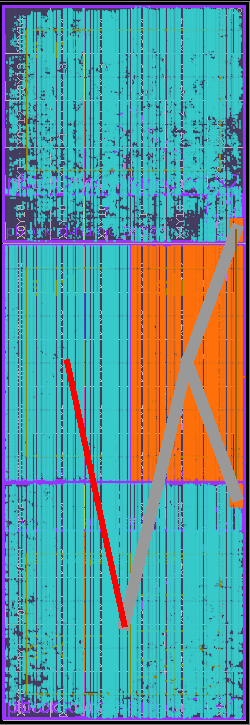
\includegraphics{box_res_int.png}
        \caption*{Netzliste für den Datentyp \texttt{int}}
    \end{minipage}\hfill
    \begin{minipage}{0.45\textwidth}
        \centering
        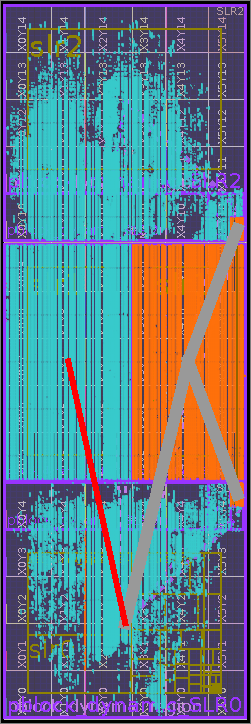
\includegraphics{box_res_float.png}
        \caption*{Netzliste für den Datentyp \texttt{float}}
    \end{minipage}
    \pdfimageresolution=72
    \caption[Netzliste des synthetisierten Box-Filter-Kernels mit verschiedenen
             Datentypen]{Netzliste des Box-Filter-Kernels mit verschiedenen
             Datentypen. Die unterschiedliche Auslastung der
             Hardware"=Ressourcen ist in dieser Ansicht deutlich sichtbar. Blaue
             Bereiche werden für die Schaltung verwendet, dunkelgraue sind nicht
             in Gebrauch. Der orange Bereich ist für die Laufzeitumgebung
             reserviert. Die kräftigen grauen und roten Balken repräsentieren
             die Zahl der Verbindungen zwischen den einzelnen
             FPGA"=Komponenten.}
    \label{ergebnisse:box:messung:netzliste}
\end{figure}

\subsubsection{Laufzeiten}

Über die in SYCL vorhandenen Profiling"=Funktionen lassen sich Erkenntnisse über
die Laufzeit gewinnen. Unglücklicherweise war nur die \texttt{float}"=Schaltung
auf dem FPGA"=Knoten lauffähig. Diese benötigte für die Filterung von
512 Bildern etwa \SI{22.26}{\second}, oder ca. \SI{45}{\milli\second} pro Bild.
Das entspricht einer Verarbeitungsfrequenz von rund 23 Bildern pro Sekunde,
womit ungefähr die Geschwindigkeit der Intel"=GPU bei der Ausführung des
\textit{jungfrau"=photoncounter} im vorigen Abschnitt erreicht ist. Für einen
Beschleuniger, der für den Einsatz in Rechenzentren ausgelegt wurde, ist das
deutlich zu wenig. Es gilt allerdings zu bedenken, dass die Synthesewerkzeuge
aufgrund des Entwicklungsstandes der Xilinx"=SYCL"=Implementierung keinerlei
Optimierungen -- wie z.B. die Nutzung des Block RAM oder Pipelining -- vornehmen
konnten, obwohl diese im Kernel"=Quelltext selbst eingefügt wurden. Mit
zunehmendem Reifegrad der Xilinx"=SYCL"=Implementierung dürfte derselbe
Quelltext zukünftig deutlich bessere Ergebnisse liefern.

Die \texttt{int}"=Schaltung führte dagegen -- trotz vorheriger Verifizierung
durch Software"= und Hardware"=Emulation -- entweder zu einem Absturz des
gesamten Knotens oder wurde vom HPC"=System nach einer Stunde(!) beendet, ohne
ein Ergebnis zu produzieren. Daher ist ein Vergleich der Laufzeiten zwischen
den Schaltungen für verschiedene Datentypen zum aktuellen Zeitpunkt nicht
möglich.
